%-------------------------------------------------------------------------------
\subsubsection{Modèle de Lotka-Volterra avec densité dépendance} 
%-------------------------------------------------------------------------------

\paragraph{Rappel.}
En notant 
\begin{itemize}
  \item $x(t)$ une variable proportionnelle au nombre de proies et
  \item $y(t)$ une variable proportionnelle au nombre de prédateurs,
\end{itemize}
le modèle Lotka-Volterra classique s'écrit, 
\begin{equation} \label{eq:LV}
\left\{\begin{array}{rcr}
        \dot x & = & r x (1 - y), \\ 
        \dot y & = & - m y (1 - x).
        \end{array}\right.
\end{equation}
Notamment, ce modèle admet deux points d'équilibre en $(x=0, y=0)$ et $(x=1, y=1)$.

\paragraph{Prise en compte d'une densité-dépendance.}
On considère ici un modèle de Lotka-Volterra avec densité dépendance. Plus précisément, en supposant le taux de croissance des proies égale à 1 ($r = 1$), on pose le modèle
\begin{equation} \label{eq:LVDD}
\left\{\begin{array}{rcr}
        \dot x & = & x (1 - y - ax), \\ 
        \dot y & = & - m y (1 - x), 
        \end{array}\right.
\end{equation}
où les paramètres $m$ et $a$ sont strictement positifs. 
% On remarque que le cas $a=0$ correspond au modèle de Lotka-Volterra classique (avec $r=1$).

\paragraph{Interprétation du modèle \eqref{eq:LVDD}.}
\begin{enumerate}
  \item Interpréter les paramètres $m$ et $a$ du modèle \eqref{eq:LVDD}.
  \solution{$m$ est le taux de mort des prédateurs en absence de proies (si $x(0)= 0$, $y(t) = y_0 e^{-mt}$). $a$ rend compte de la compétition entre les proies, c'est-à-dire de la limitation des ressources du milieu.}
  \item Déterminer les points d'équilibre du système \eqref{eq:LVDD}.
  \solution{
  L'isocline $\{\dot x = 0\}$ est $\Ical_x = \{x = 0\} \cup \{y = 1 - ax\}$ et l'isocline $\{\dot y = 0\}$ est $\Ical_y = \{y = 0\} \cup \{x = 1\}$. Les points d'équilibre sont donc $(0, 0)$, $(0, 1/a)$ et $(1, 1-a)$.}
  \item Expliquer la position du point d'équilibre $(x^*, y^*)$ non nul (c'est-à-dire pour lequel $x^*$ et $y^*$ sont non nuls) par rapport au point d'équilibre non nul du modèle de Lotka-Volterra classique \eqref{eq:LV}.
  \solution{L'équilibre non-trivial du modèle de Lotka-Volterra est le point $(1, 1)$. Le point d'équilibre des proies est conservé ($x^* = 1$), mais celui des prédateurs diminue $y^* = 1-a < 1$ : la contrainte imposée par le milieu au proies nuit, {\it in fine} à la population des prédateurs.}
\end{enumerate}

\bigskip
\paragraph{Questions intermédiaires (I).}
Soit la fonction $f: \Rbb^{*+} \mapsto \Rbb$, définie par $f(x) = \sqrt{x(x+1)} - x$.
\begin{enumerate}
  \setcounter{enumi}{3}
  \item Montrer que $f(x) > 0$. \label{q:LVDD-f1}
  \solution{On a $\sqrt{x(x+1)} > \sqrt{x^2} = x$, donc $f(x) > 0$.
  }
  \item Montrer que $f(x) < 1/2$. \label{q:LVDD-f2}
  \solution{On a
  $$
  f(x) < \frac12 
  \qquad \Leftrightarrow \qquad
  x(x+1) < \left(x + \frac12\right)^2
  \qquad \Leftrightarrow \qquad
  x^2 + x < x^2 + x + \frac14
  $$
  qui est toujours vrai.
  }
\end{enumerate}

\paragraph{Questions intermédiaires (II).}
Soit la matrice $J^*$ définie par
\begin{equation} \label{eq:LVDD-Jstar}
  J^* = \left(\begin{array}{cc}
              -a & -1 \\ m(1-a) & 0
              \end{array}\right).
\end{equation}

\bigskip
\begin{enumerate}
  \setcounter{enumi}{5}
  \item Déterminer le polynôme caractéristique $P$ de $J^*$.
  \solution{$P(\lambda) = \lambda^2 + a \lambda + m(1-a)$.}
  %
  \item Montrer que les valeurs propres de $J^*$ sont réelles si et seulement si $a \geq a_1 = 2 f(m)$, où $f$ est la fonction définie en (I). 
  ({\sl On pourra étudier le discriminant $\Delta$ de $P$ comme une fonction de $a$.})
  \solution{La nature des valeurs propres de $J^*$ est donnée par le signe du discriminant de $P$ : $\Delta = \Delta(a) = a^2 + 4am - 4m$ qui est lui même un polynôme en $a$. \\
  Son discriminant est $\delta = 16m^2 + 16m = 16 m(m+1)$ est positif puisque $m$ est positif. 
  $\Delta(a)$ admet donc deux racines réelles:  $-2 (m + \sqrt{m(m+1)})$, qui est négative, et $a_1 = 2 (\sqrt{m(m+1)} - m) = 2f(m)$ qui est strictement positive d'après la question \ref{q:LVDD-f1}. 
  \\ $\Delta(a)$ est donc positif dès que $a \geq a_1 = 2 f(m)$ et $P$ admet alors deux racines réelles (égales si $a = a_1$). 
  }
  %
  \item Montrer que $a_1 < 1$ et que si $a > 1$, les valeurs propres de $J^*$ sont de signes différents. \label{q:racinePstar}
  \solution{
  La question \ref{q:LVDD-f2} nous assure que $a_1 = 2 f(m) < 1$, puisque $f(x) < 1/2$ pour tout $x \geq 0$. \\
  Si $a > a_1$, $P$ admet pour racines réelles $\lambda_1 = -(a +\sqrt{\Delta(a)})/2$, qui est toujours négative, et $\lambda_2 = (-a + \sqrt{\Delta(a)})/2$, qui est est positive dès que 
  $$
  \sqrt{\Delta(a)} \geq a
  \qquad \Leftrightarrow \qquad
  a^2 + 4am - 4m \geq a^2
  \qquad \Leftrightarrow \qquad
  a \geq 1.
  $$
  $J^*$ a donc des valeurs propres de racines distinctes dès que $a > 1 > a_1$. \\ 
  Alternativement, par les propriétés du polynôme caractéristique d'une matrice de $\Mcal_2$, $\lambda_1$ et $\lambda_2$ sont de même signe ssi $\lambda_1 \lambda_2 = |J^*| = m(1-a) > 0$, c'est-à-dire si $a <1$, puisque $m > 0$.
  }
\end{enumerate}
  

\paragraph{Stabilité du point d'équilibre non nul.}
On s'intéresse maintenant à la stabilité du point d'équilibre $(x^*, y^*)$ non nul. 
\begin{enumerate}
  \setcounter{enumi}{8}
  \item Déterminer la matrice jacobienne du système en un point $(x, y)$ quelconque.
  \solution{
  $$
  J = \left(\begin{array}{cc}
            -2ax + (1-y) & -x \\ my & m(x-1) 
            \end{array}\right).
  $$
  }
  \item En déduire que la matrice jacobienne en $(x^*, y^*)$ est égale à la matrice $J^*$ définie à l'équation \eqref{eq:LVDD-Jstar}.
  \solution{Direct.}
  \item \'Etudier la nature de l'équilibre $(x^*, y^*)$ en fonction de la position de $a$ par rapport aux deux valeurs seuils $a_1$ et $1$ : $a < a_1$, $a_1 < a < 1$ ou $a > 1$.
  ({\sl On ne s'attardera pas sur les cas limites $a = a_1$ et $a = 1$}.)
  \solution{
  \begin{description}
    \item[$a < a_1$ :] dans ce cas, $\Delta(a) < 0$ et les valeurs propres de $J*$ sont $\lambda_1$ et $\lambda_2$ calculées à la question \ref{q:racinePstar}, qui sont complexes mais dont les parties réelles sont négatives puisque $a > 0$. L'équilibre $(x^*, y^*)$ est donc un équilibre stable.
    \item[$a_1 < a < 1$ :] dans ce cas, $\Delta(a) > 0$ et les valeurs propres $\lambda_1$ et $\lambda_2$ sont toutes les deux réelles et négatives : l'équilibre $(x^*, y^*)$ est donc toujours stable.
    \item[$a > 1$ :] $\lambda_1$ est toujours négative mais $\lambda_2$ devient positive et $(x^*, y^*)$ devient alors instable.
  \end{description}
  Les figures suivantes donnent respectivement les parties réelles $Re(\lambda)$ et imaginaires $Im(\lambda)$  des valeurs propres $\lambda_1$ et $\lambda_2$ en fonction de $a$ pour $m=1/2$. 
  $$
  \begin{array}{c}
    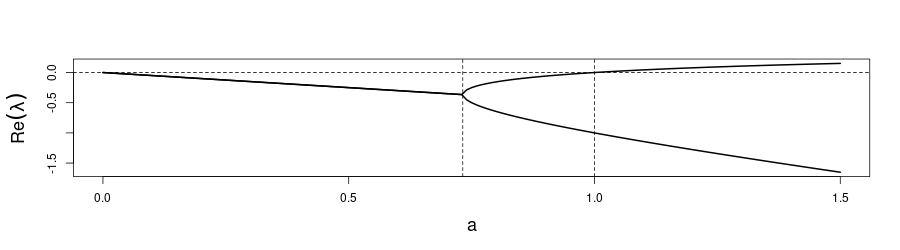
\includegraphics[width=.8\textwidth, trim=0 0 0 50, clip=]{LotkaVolterraDD-m0.5-eigenValueReal.png} \\
    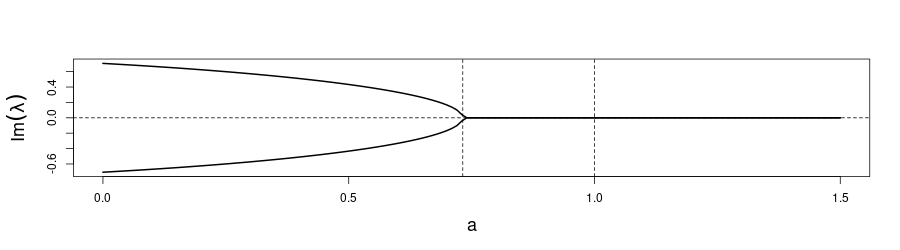
\includegraphics[width=.8\textwidth, trim=0 0 0 50, clip=]{LotkaVolterraDD-m0.5-eigenValueImaginary.png} 
  \end{array}
  $$
  La bifurcation se produit en $a = a_1$ et l'une des valeurs propres devient positive pour $a = 1$.
  }
\end{enumerate}

\paragraph{Trajectoires.}
Les trajectoires ($i$), ($ii$) et ($iii$) suivantes ont été obtenues par intégration numérique avec $m = 1/2$ et partant de l'état initial $(x_0 = 2,\;  y_0 = 3/2)$ pour trois valeurs de $a$ différentes :
$$
\begin{array}{ccc}
  (i) & (ii) & (iii) \\
  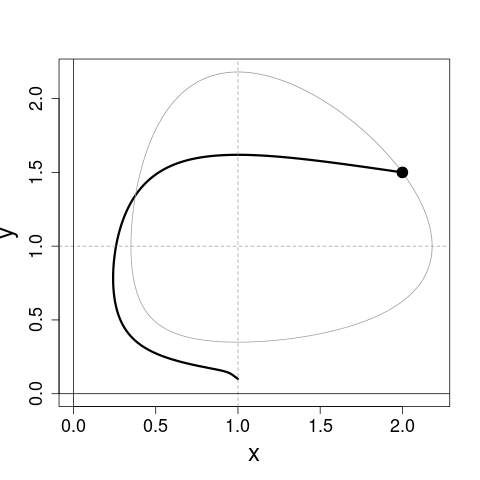
\includegraphics[width=.32\textwidth, trim=0 0 0 50, clip=]{LotkaVolterraDD-m0.5-a0.9.png} &
  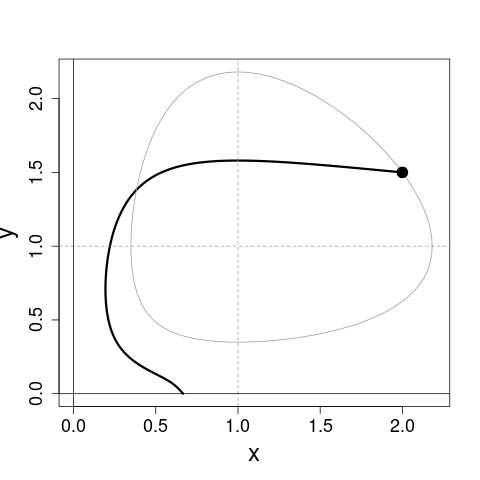
\includegraphics[width=.32\textwidth, trim=0 0 0 50, clip=]{LotkaVolterraDD-m0.5-a1.5.png} &
  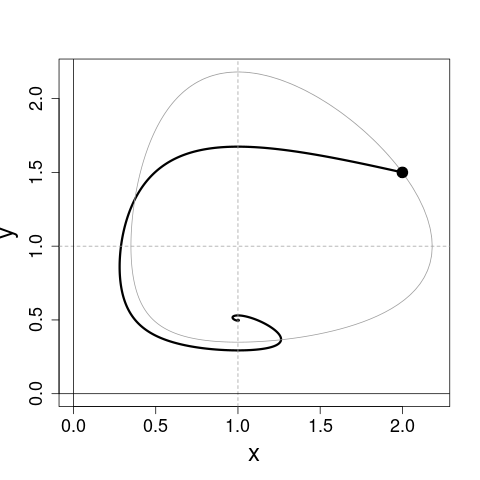
\includegraphics[width=.32\textwidth, trim=0 0 0 50, clip=]{LotkaVolterraDD-m0.5-a0.5.png}
\end{array}
$$
La courbe grise indique la trajectoire du modèle de Lotka-Volterra \eqref{eq:LV} sans densité-dépendance ($m = 1/2$, $a = 0$), partant du même point initial. Les repères grisés indiquent le point d'équilibre de ce même modèle \eqref{eq:LV}.

\begin{enumerate}
  \setcounter{enumi}{11}
  \item Associer chacune des trajectoires ($i$), ($ii$) et ($iii$) à l'une des trois valeurs de $a$ : $a = 1/2$, $a = 9/10$ et $a = 3/2$.
  \solution{On a dans ce cas $a_1 = 2 f(1/2) = \sqrt{3} - 1 \simeq 0.73$.
  \begin{description}
    \item[$a = 1/2 < a_1$ :] le système possède un équilibre stable en ($x^* = 1, y^* = 1/2$) et les valeurs propres de $J^*$ possèdent une partie imaginaire non nulle qui induit un enroulement autour de l'équilibre : on reconnaît la trajectoire ($iii$).
    \item[$a_1 < a = 9/10 < 1$ :] le système possède un équilibre stable en ($x^* = 1, y^* = 1/10$) mais les valeurs propres de $J^*$ sont réelles et négatives : le système tend vers l'équilibre sans enroulement : on reconnaît la trajectoire ($i$).
    \item[$a = 3/2 > a_1$ :] le système possède un équilibre instable en ($x^* = 1, y^* = -1/2$) que le système n'atteint jamais, du fait de l'extinction des prédateurs ($y(t) \to 0$) : on reconnaît la trajectoire ($ii$).
  \end{description}
  }
  \item Donner la limite de $x(t)$ quand $t$ tend vers l'infini dans le cas ($ii$).
  \solution{
  Dans ce cas, $y(t)$ tend vers 0 quand $t \to\infty$, le système \eqref{eq:LVDD-Jstar} devient donc simplement $\dot x = F(x)$ avec $F(x) = x (1 - ax)$. Ce système admet deux points d'équilibre en $x_1 = 0$ et $x_2 = 1/a$ et seul le second est stable (car $F'(x_1) > 0$ et $F'(x_2) < 0$). \\
  Après extinction des prédateurs, la population des proies tend donc vers un des équilibres 'nuls' : $(x_2 = 1/a = 2/3, y=0)$. Du fait de la densité-dépendance, la population des proies n'explose donc pas, contrairement au modèle de Lotka-Volterra classique.
  }
\end{enumerate}
